% !TeX root = ../main.tex
\documentclass[./../main.tex]{subfiles}

\begin{document}

\subsection{Kiến trúc}

Hình \ref{fig:high_level_design} mô tả thiết kế bậc cao của hệ thống UETWork mới. Hệ thống bao gồm 4 thành phần chính:

\begin{itemize}
	\item

	      \textbf{Web App}: là ứng dụng web mà người dùng tương tác để hoàn
	      thành công việc của mình.

	\item

	      \textbf{API Gateway}: nhận yêu cầu HTTP từ client, gửi yêu cầu tới
	      những service cần thiết, sau đó tổng hợp lại response để trả lại kết
	      quả cho client.

	\item

	      \textbf{User Service}: xử lý yêu cầu liên quan đến account và profile
	      của người dùng trên hệ thống, bao gồm sinh viên, giảng viên, đối tác,
	      \ldots{} cùng với thông tin về các khoa. Service này nhận yêu cầu bằng
	      giao thức gRPC và HTTP (cho API upload file).

	\item

	      \textbf{Internship Service}: xử lý yêu cầu liên quan đến kỳ thực tập,
	      ví dụ như danh sách kỳ thực tập, các sinh viên trong kỳ, \ldots{}
	      Service này sẽ replicate lại một số data từ User Service để đảm bảo
	      tính đúng đắn và toàn vẹn của dữ liệu. Service này nhận yêu cầu bằng
	      giao thức gRPC\cite{Goo22} và HTTP (cho API upload file).

\end{itemize}

Ngoài 4 thành phần chính ở trên, hệ thống có các thành phần phụ là:

\begin{itemize}
	\item

	      \textbf{Debezium}: đọc bản ghi từ cơ sở dữ liệu của User Service,
	      chuyển bản ghi đó thành Kafka message và gửi vào Kafka.

	\item

	      \textbf{Internship Service Replicator}: đọc bản ghi của User DB từ
	      Kafka và insert vào Internship DB.

\end{itemize}

\begin{figure}
	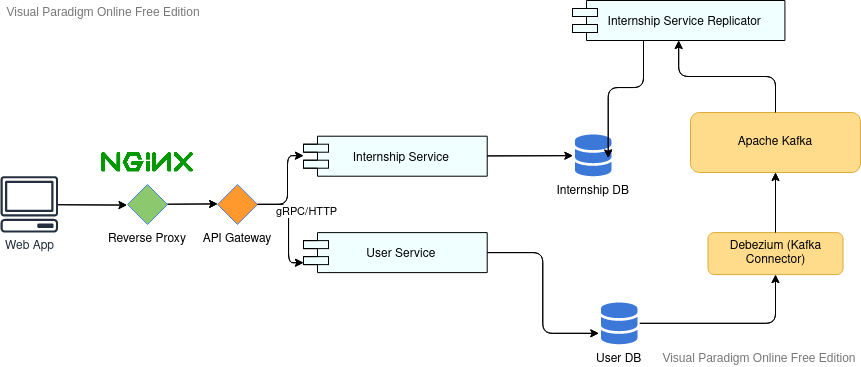
\includegraphics[width=\linewidth]{./images/uetwork_architecture.png}
	\caption{Thiết kế bậc cao}
	\label{fig:high_level_design}
\end{figure}

\subsection{Thiết kế cơ sở dữ liệu}

Hệ thống UETWork có 2 service chính: User Service và Internship Service. Mỗi service có nhiệm vụ tự quản lý dữ liệu của mình. Dưới đây là lược đồ cơ sở dữ liệu cho 2 service này.

\subsubsection{Cơ sở dữ liệu của User Service (User DB)}

Hình \ref{fig:user_db_design} mô tả các bảng và mối quan hệ giữa chúng trong User DB. Bảng \ref{tab:db_roles} đến \ref{tab:db_partner_orgs} mô tả cụ thể hơn về nội dung từng bảng trong User DB.

\begin{figure}
	\centering
	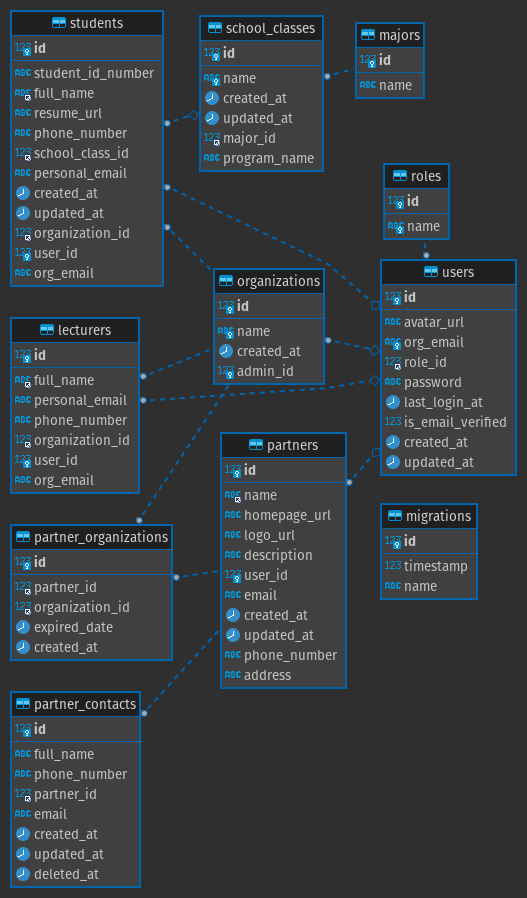
\includegraphics[width=0.7\linewidth]{./images/image3.png}
	\caption{Lược đồ User DB}
	\label{fig:user_db_design}
\end{figure}

\begin{table}[H]
	\caption[Bảng roles]{Bảng \textbf{roles} - chứa thông tin về các role (vai trò)}
	\label{tab:db_roles}
	\begin{tabular}{|l|l|l|}
		\hline
		\textbf{Tên cột} & \textbf{Kiểu dữ liệu} & \textbf{Mô tả} \\ \hline
		id               & int                   & Mã định danh   \\ \hline
		name             & varchar               & Tên của role   \\ \hline
		phone\_number    & varchar               & Số điện thoại  \\ \hline
	\end{tabular}
\end{table}

\begin{table}[H]
	\caption[Bảng users]{Bảng \textbf{users} - chứa thông tin về tài khoản người dùng}
	\label{tab:db_users}
	\begin{tabularx}{\textwidth}{|l|l|X|}
		\hline
		\textbf{Tên cột}    & \textbf{Kiểu dữ liệu} & \textbf{Mô tả}                                         \\ \hline
		id                  & int                   & Mã định danh                                           \\ \hline
		avatar\_url         & varchar               & Địa chỉ avatar của người dùng                          \\ \hline
		org\_email          & varchar               & Địa chỉ email để người dùng đăng nhập                  \\ \hline
		role\_id            & int                   & Mã định danh của role                                  \\ \hline
		password            & varchar               & Mật khẩu đã được băm bằng thuật toán bcrypt            \\ \hline
		last\_login\_at     & timestamp             & Thời gian đăng nhập thành công gần nhất của người dùng \\ \hline
		is\_email\_verified & boolean               & Email người dùng đã được xác nhận hay chưa?            \\ \hline
		created\_at         & timestamp             & Thời gian tạo                                          \\ \hline
		updated\_at         & timestamp             & Thời gian cập nhật gần nhất                            \\ \hline
	\end{tabularx}
\end{table}

\begin{table}[H]
	\caption[Bảng organizations]{Bảng \textbf{organizations} - chứa thông tin về các khoa}
	\label{tab:db_organizations}
	\begin{tabular}{|l|l|l|}
		\hline
		\textbf{Tên cột} & \textbf{Kiểu dữ liệu} & \textbf{Mô tả}                      \\ \hline
		id               & int                   & Mã định danh                        \\ \hline
		name             & varchar               & Tên khoa                            \\ \hline
		admin\_id        & int                   & Mã định danh của quản trị viên khoa \\ \hline
		created\_at      & timestamp             & Thời gian tạo                       \\ \hline
	\end{tabular}
\end{table}

\begin{table}[H]
	\caption[Bảng school\_classes]{Bảng \textbf{school\_classes} - chứa thông tin về lớp khóa học}
	\label{tab:db_school_classes}
	\begin{tabular}{|l|l|l|}
		\hline
		\textbf{Tên cột} & \textbf{Kiểu dữ liệu} & \textbf{Mô tả}           \\ \hline
		id               & int                   & Mã định danh             \\ \hline
		name             & varchar               & Tên lớp khóa học         \\ \hline
		program\_name    & varchar               & Tên chương trình đào tạo \\ \hline
	\end{tabular}
\end{table}

\begin{table}[H]
	\caption[Bảng students]{Bảng \textbf{students} - chứa thông tin về profile sinh viên}
	\label{tab:db_students}
	\begin{tabularx}{\textwidth}{|l|l|X|}
		\hline
		\textbf{Tên cột}    & \textbf{Kiểu dữ liệu} & \textbf{Mô tả}                        \\ \hline
		id                  & int                   & Mã định danh                          \\ \hline
		student\_id\_number & varchar               & Mã số sinh viên (được nhà trường cấp) \\ \hline
		full\_name          & varchar               & Họ tên đầy đủ                         \\ \hline
		resume\_url         & varchar               & Địa chỉ lưu trữ CV của người dùng     \\ \hline
		phone\_number       & varchar               & Số điện thoại của người dùng          \\ \hline
		school\_class\_id   & int                   & Mã định danh lớp học của sinh viên    \\ \hline
		personal\_email     & varchar               & Địa chỉ email cá nhân của sinh viên   \\ \hline
		created\_at         & timestamp             & Thời gian tạo                         \\ \hline
		updated\_at         & timestamp             & Thời gian cập nhật gần nhất           \\ \hline
		organization\_id    & int                   & Mã định danh khoa của sinh viên       \\ \hline
		user\_id            & int                   & Mã định danh tài khoản                \\ \hline
		org\_email          & varchar               & Email VNU                             \\ \hline
	\end{tabularx}%
\end{table}

\begin{table}[H]
	\caption[Bảng lecturers]{Bảng \textbf{lecturers} - chứa thông tin về profile giảng viên}
	\label{tab:db_lecturers}
	\begin{tabular}{|l|l|l|}
		\hline
		\textbf{Tên cột} & \textbf{Kiểu dữ liệu} & \textbf{Mô tả}          \\ \hline
		id               & int                   & Mã định danh            \\ \hline
		full\_name       & varchar               & Họ tên đầy đủ           \\ \hline
		org\_email       & varchar               & Địa chỉ email VNU       \\ \hline
		personal\_email  & varchar               & Địa chỉ email cá nhân   \\ \hline
		phone\_number    & varchar               & Số điện thoại           \\ \hline
		organization\_id & int                   & Mã định danh khoa       \\ \hline
		user\_id         & int                   & Mã định danh người dùng \\ \hline
	\end{tabular}%
\end{table}

\begin{table}[H]
	\caption[Bảng partners]{Bảng \textbf{partners} - chứa thông tin về profile công ty trong hệ thống}
	\label{tab:db_partners}
	\begin{tabularx}{\textwidth}{|l|l|X|}
		\hline
		\textbf{Tên cột} & \textbf{Kiểu dữ liệu} & \textbf{Mô tả}                               \\ \hline
		id               & int                   & Mã định danh                                 \\ \hline
		name             & varchar               & Tên công ty                                  \\ \hline
		homepage\_url    & varchar               & Địa chỉ trang chủ công ty                    \\ \hline
		logo\_url        & varchar               & Địa chỉ logo công ty                         \\ \hline
		description      & varchar               & Mô tả công ty                                \\ \hline
		user\_id         & int                   & Mã định danh người dùng                      \\ \hline
		email            & varchar               & Địa chỉ email của bộ phận tuyển dụng công ty \\ \hline
		created\_at      & timestamp             & Thời gian tạo                                \\ \hline
		updated\_at      & timestamp             & Thời gian cập nhật gần nhất                  \\ \hline
		phone\_number    & varchar               & Số điện thoại                                \\ \hline
		address          & varchar               & Địa chỉ công ty                              \\ \hline
		org\_email       & varchar               & Email VNU                                    \\ \hline
	\end{tabularx}
\end{table}

\begin{table}[H]
	\caption[Bảng partner\_contacts]{Bảng \textbf{partner\_contacts} - chứa thông tin về liên hệ của đối tác}
	\label{tab:db_partner_contacts}
	\begin{tabular}{|l|l|l|}
		\hline
		\textbf{Tên cột} & \textbf{Kiểu dữ liệu} & \textbf{Mô tả}              \\ \hline
		id               & int                   & Mã định danh                \\ \hline
		full\_name       & varchar               & Họ tên đầy đủ               \\ \hline
		phone\_number    & varchar               & Số điện thoại               \\ \hline
		partner\_id      & int                   & Mã định danh công ty        \\ \hline
		email            & varchar               & Địa chỉ email của liên hệ   \\ \hline
		created\_at      & timestamp             & Thời gian tạo               \\ \hline
		updated\_at      & timestamp             & Thời gian cập nhật gần nhất \\ \hline
		deleted\_at      & timestamp             & Thời gian liên hệ bị xóa    \\ \hline
	\end{tabular}
\end{table}

\begin{table}[H]
	\caption[Bảng partner\_organizations]{Bảng \textbf{partner\_organizations} - chứa trạng thái liên kết giữa công ty và khoa}
	\label{tab:db_partner_orgs}
	\begin{tabular}{|l|l|l|}
		\hline
		\textbf{Tên cột} & \textbf{Kiểu dữ liệu} & \textbf{Mô tả}                       \\ \hline
		id               & int                   & Mã định danh                         \\ \hline
		partner\_id      & int                   & Mã định danh công ty                 \\ \hline
		organization\_id & int                   & Mã định danh khoa                    \\ \hline
		expired\_date    & date                  & Thời gian kết thúc hợp đồng liên kết \\ \hline
		created\_at      & timestamp             & Thời gian tạo                        \\ \hline
	\end{tabular}
\end{table}

Bảng \textbf{migrations} chứa thông tin liên quan đến migration của cơ sở dữ liệu. Không liên quan tới chức năng của hệ thống

\subsubsection{Cơ sở dữ liệu của Internship Service}

Hình \ref{fig:internship_db_design} mô tả thiết kế của Internship DB. Cơ sở dữ liệu này đã nhân bản lại một số bảng từ User DB để giúp việc query dễ dàng hơn. Các bảng được nhân bản từ User DB bao gồm:

\begin{itemize}
	\item

	      Bảng students

	\item

	      Bảng lecturers

	\item

	      Bảng partners

	\item

	      Bảng partner\_contacts

	\item

	      Bảng organizations

	\item

	      Bảng partner\_organizations

	\item

	      Bảng school\_classes

\end{itemize}

Bảng \ref{tab:db_terms} đến \ref{tab:db_posts} mô tả nội dung cụ thể của từng bảng trong cơ sở dữ liệu Internship DB.

\begin{figure}
	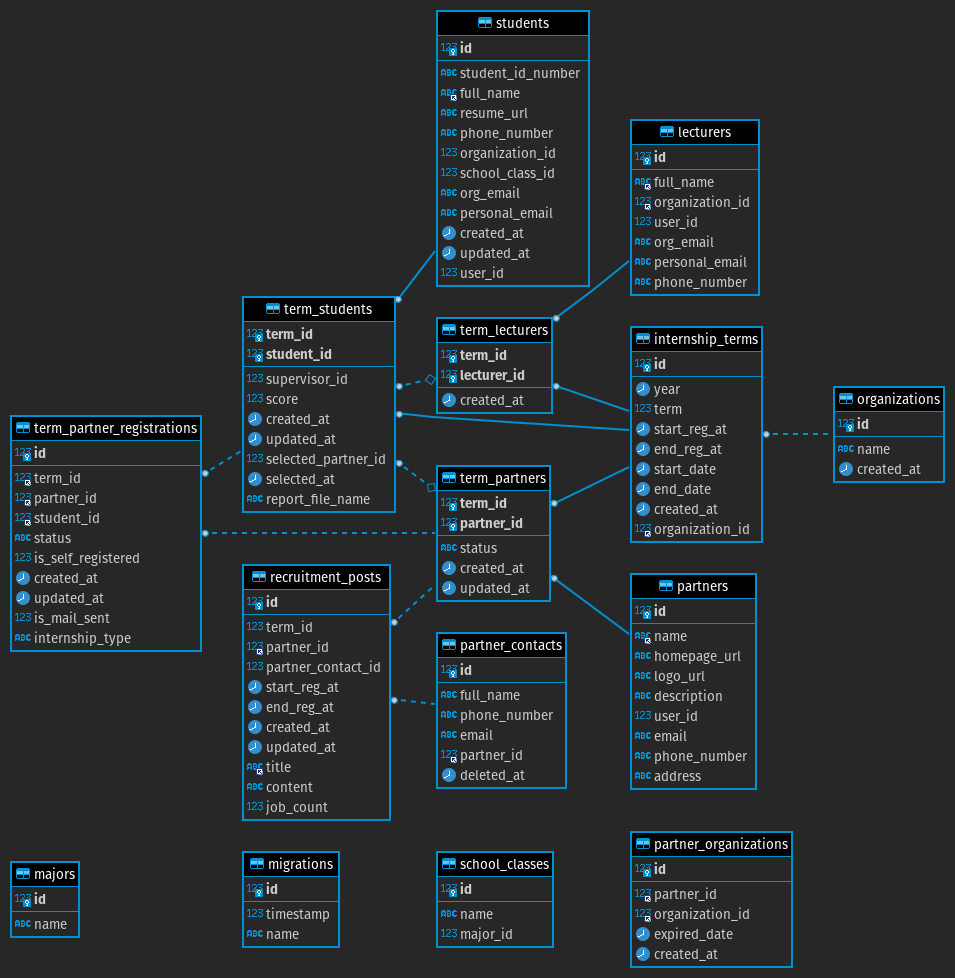
\includegraphics[width=\linewidth]{./images/image1.png}
	\caption{Lược đồ Internship DB}
	\label{fig:internship_db_design}
\end{figure}

\begin{table}[H]
	\caption[Bảng internship\_terms]{Bảng \textbf{internship\_terms} - chứa kỳ thực tập của các khoa}
	\label{tab:db_terms}
	\begin{tabular}{|l|l|l|}
		\hline
		\textbf{Tên cột} & \textbf{Kiểu dữ liệu} & \textbf{Mô tả}                     \\ \hline
		id               & int                   & Mã định danh                       \\ \hline
		year             & year                  & Năm của kỳ thực tập                \\ \hline
		term             & int                   & Đợt của kỳ thực tập (v.d. 1, 2, 3) \\ \hline
		start\_reg\_at   & timestamp             & Thời gian bắt đầu đăng ký          \\ \hline
		end\_reg\_at     & timestamp             & Thời gian kết thúc đăng ký         \\ \hline
		start\_date      & date                  & Ngày bắt đầu kỳ thực tập           \\ \hline
		end\_date        & date                  & Ngày kết thúc kỳ thực tập          \\ \hline
		created\_at      & timestamp             & Thời gian tạo                      \\ \hline
		organization\_id & int                   & Mã định danh khoa                  \\ \hline
	\end{tabular}
\end{table}

\begin{table}[H]
	\caption[Bảng term\_students]{Bảng \textbf{term\_students} - chứa thông tin thực tập của toàn bộ sinh viên}
	\label{tab:db_term_students}
	\begin{tabular}{|l|l|l|}
		\hline
		\textbf{Tên cột}      & \textbf{Kiểu dữ liệu} & \textbf{Mô tả}                       \\ \hline
		term\_id              & int                   & Mã định danh kỳ thực tập             \\ \hline
		student\_id           & int                   & Mã định danh sinh viên               \\ \hline
		supervisor\_id        & int                   & Mã định danh giảng viên hướng dẫn    \\ \hline
		score                 & int                   & Điểm                                 \\ \hline
		created\_at           & timestamp             & Thời gian tạo                        \\ \hline
		updated\_at           & timestamp             & Thời gian cập nhật gần nhất          \\ \hline
		selected\_partner\_id & int                   & Mã định danh công ty được chọn       \\ \hline
		selected\_at          & timestamp             & Thời gian chọn công ty               \\ \hline
		report\_file\_name    & varchar               & Địa chỉ lưu trữ file báo cáo cuối kỳ \\ \hline
	\end{tabular}
\end{table}



\begin{table}[H]
	\caption[Bảng term\_lecturers]{Bảng \textbf{term\_lecturers} - chứa thông tin thực tập của giảng viên}
	\label{tab:db_term_lecturers}
	\begin{tabular}{|l|l|l|}
		\hline
		\textbf{Tên cột} & \textbf{Kiểu dữ liệu} & \textbf{Mô tả}           \\ \hline
		term\_id         & int                   & Mã định danh kỳ thực tập \\ \hline
		lecturer\_id     & int                   & Mã định danh giảng viên  \\ \hline
		created\_at      & timestamp             & Thời gian tạo            \\ \hline
	\end{tabular}
\end{table}


\begin{table}[H]
	\caption[Bảng term\_partners]{Bảng \textbf{term\_partners} - chứa thông tin của công ty trong kỳ thực tập}
	\label{tab:db_term_partners}
	\begin{tabularx}{\textwidth}{|l|X|X|}
		\hline
		\textbf{Tên cột} & \textbf{Kiểu dữ liệu}                   & \textbf{Mô tả}                                               \\ \hline
		term\_id         & int                                     & Mã định danh kỳ thực tập                                     \\ \hline
		partner\_id      & int                                     & Mã định danh công ty                                         \\ \hline
		status           & enum(‘ACCEPTED', ‘PENDING', ‘REJECTED’) & Trạng thái công ty (được chấp nhận / chờ duyệt / bị từ chối) \\ \hline
		created\_at      & timestamp                               & Thời gian tạo                                                \\ \hline
		updated\_at      & timestamp                               & Thời gian cập nhật gần nhất                                  \\ \hline
	\end{tabularx}
\end{table}


\begin{table}[H]
	\caption[Bảng term\_partner\_registrations]{Bảng \textbf{term\_partner\_registrations} - chứa thông tin đăng ký thực tập của sinh viên}
	\label{tab:db_term_partner_regs}
	\begin{tabularx}{\textwidth}{|l|X|X|}
		\hline
		\textbf{Tên cột}     & \textbf{Kiểu dữ liệu}                           & \textbf{Mô tả}                                 \\ \hline
		id                   & int                                             & Mã định danh                                   \\ \hline
		term\_id             & int                                             & Mã định danh kỳ thực tập                       \\ \hline
		student\_id          & int                                             & Mã định danh sinh viên                         \\ \hline
		partner\_id          & int                                             & Mã định danh công ty                           \\ \hline
		status               & enum(‘PASSED', ‘FAILED', ‘SELECTED', ‘WAITING') & Kết quả phỏng vấn                              \\ \hline
		is\_self\_registered & boolean                                         & Có phải sinh viên này đã tự đăng ký không?     \\ \hline
		created\_at          & timestamp                                       & Thời gian tạo                                  \\ \hline
		updated\_at          & timestamp                                       & Thời gian cập nhật gần nhất                    \\ \hline
		is\_mail\_sent       & boolean                                         & Mail thông báo đã được gửi hay chưa?           \\ \hline
		internship\_type     & enum(‘ASSOCIATE’, ‘OTHER')                      & Loại thực tập (thực tập đối tác/công ty ngoài) \\ \hline
	\end{tabularx}
\end{table}

\begin{table}[H]
	\caption[Bảng recruitment\_posts]{Bảng \textbf{recruitment\_posts} - chứa bài đăng tuyển dụng trong 1 kỳ thực tập}
	\label{tab:db_posts}
	\begin{tabular}{|l|l|l|}
		\hline
		\textbf{Tên cột}     & \textbf{Kiểu dữ liệu} & \textbf{Mô tả}                   \\ \hline
		id                   & int                   & Mã định danh                     \\ \hline
		term\_id             & int                   & Mã định danh kỳ thực tập         \\ \hline
		partner\_id          & int                   & Mã định danh công ty             \\ \hline
		partner\_contact\_id & int                   & Mã định danh liên hệ của đối tác \\ \hline
		start\_reg\_at       & timestamp             & Ngày bắt đầu đăng ký             \\ \hline
		end\_reg\_at         & timestamp             & Ngày kết thúc đăng ký            \\ \hline
		title                & varchar               & Tiêu đề bài đăng                 \\ \hline
		content              & varchar               & Nội dung bài đăng                \\ \hline
		job\_count           & int                   & Số người cần tuyển               \\ \hline
	\end{tabular}
\end{table}

\subsection{Thiết kế API}

HTTP API\footnote{\url{https://uetwork.stoplight.io/}} của Gateway được thiết kế theo mô hình REST API. Nói chung, một endpoint chỉ có thể được truy cập bởi 1 role duy nhất và có 1 schema cố định. Điều này giúp cho nhà phát triển bên máy khách dễ tích hợp API, cũng như tránh nhầm lẫn trong quá trình này.

gRPC API của User Service và Internship Service được định nghĩa bằng file \code{.proto}\footnote{\url{https://gitlab.com/laituananh1711/intern-management/-/tree/master/proto}} trong mã nguồn hệ thống. Với các endpoint để upload file, hai service sử dụng HTTP do gRPC không hỗ trợ tốt với file có kích thước lớn.

\subsection{Các bài toán phức tạp và phương án giải quyết}

Phần này mô tả những bài toán khó em gặp phải khi cài đặt hệ thống với
kiến trúc microservice và hướng giải quyết cho những bài toán đó.

\hypertarget{cuxe1ch-ux111ux1ecdc-dux1eef-liux1ec7u-nux1eb1m-ux1edf-2-cux1a1-sux1edf-dux1eef-liux1ec7u-khuxe1c-nhau}{%
	\subsubsection{Cách đọc dữ liệu nằm ở 2 cơ sở dữ liệu khác
		nhau}\label{cuxe1ch-ux111ux1ecdc-dux1eef-liux1ec7u-nux1eb1m-ux1edf-2-cux1a1-sux1edf-dux1eef-liux1ec7u-khuxe1c-nhau}}

Một hệ thống luôn cần có khả năng đọc dữ liệu từ nhiều bảng khác nhau để
phục vụ cho những mục đích như thống kê, \ldots{} Tuy nhiên, với kiến
trúc Microservice, mỗi service sẽ sở hữu và quản lý data của mình. Vì
vậy, việc đọc từ nhiều bảng dữ liệu khác nhau trở nên khó khăn hơn, vì
các bảng có thể nằm trên 2 cơ sở dữ liệu khác nhau.

Để giải quyết vấn đề này, em đã cân nhắc những giải pháp sau:

\begin{enumerate}
	\def\labelenumi{\arabic{enumi}.}
	\item

	      Gọi API tới cả 2 service và ghép kết quả trả về thủ công

	\item

	      Nhân bản data giữa 2 service để giúp service thực hiện query trên 1 cơ
	      sở dữ liệu duy nhất

\end{enumerate}

Ưu điểm của cách 1 là sự phân chia rõ ràng trong nhiệm vụ của từng
service. Tuy nhiên, nhược điểm của cách làm này là sự phức tạp trong quá
trình đọc và ghép dữ liệu từ 2 service, cũng như tạo ra một sự phụ thuộc
giữa 2 service vào nhau.

Cách 2 có ưu điểm là service có thể query dữ liệu đơn giản hơn (vì dữ
liệu cùng nằm trong 1 cơ sở dữ liệu), đồng thời giúp 2 service chạy độc
lập hơn. Nhược điểm của cách làm này là hệ thống cần cài đặt cơ chế nhân
bản dữ liệu giữa 2 service, và cần đảm bảo dữ liệu nhân bản là chính xác
và kịp thời.

Với ưu điểm và nhược điểm kể trên, em đã chọn cách số 2 để giải quyết
vấn đề này.

\hypertarget{cuxe1ch-cuxe0i-ux111ux1eb7t-tuxednh-nux103ng-xuxe1c-thux1ef1c-vuxe0-phuxe2n-quyux1ec1n}{%
	\subsubsection{Cách cài đặt tính năng xác thực và phân
		quyền}\label{cuxe1ch-cuxe0i-ux111ux1eb7t-tuxednh-nux103ng-xuxe1c-thux1ef1c-vuxe0-phuxe2n-quyux1ec1n}}

Với hệ thống theo kiến trúc monolith, ta có thể phân quyền các route một
cách trực tiếp. Tuy nhiên, với kiến trúc Microservice, việc cài đặt phân
quyền trong từng service sẽ tăng độ phức tạp lên đáng kể.

Để giải quyết vấn đề này, nhiệm vụ xác thực được giao cho một
service duy nhất. Service này có nhiệm vụ xác thực người dùng và trả về
token. Sau đó, em bổ sung tính năng phân quyền vào API Gateway để đảm
bảo người dùng không truy cập trái phép.

Do service không cài đặt tính năng phân quyền, em đã bổ sung tính năng
xác thực bằng API Key. Chỉ những yêu cầu chứa API Key đúng mới có thể
được xử lý bởi service. Như vậy, dù service có bị expose ra ngoài thì
các bên thứ ba cũng không thể gửi request đến service được.

\hypertarget{cho-phuxe9p-nhiux1ec1u-khoa-sux1eed-dux1ee5ng-hux1ec7-thux1ed1ng}{%
	\subsubsection{Cho phép nhiều khoa sử dụng hệ
		thống}\label{cho-phuxe9p-nhiux1ec1u-khoa-sux1eed-dux1ee5ng-hux1ec7-thux1ed1ng}}

Hệ thống UETWork mới có nhiệm vụ hỗ trợ sinh viên và admin của nhiều
khoa. Vì vậy, một giải pháp cần được thiết kế để phân tách dữ liệu của các
khoa, đảm bảo rằng các khoa không thể đọc dữ liệu của nhau.

Vấn đề này có 2 giải pháp sau:

\begin{itemize}
	\item

	      Tạo ra một service mới là Organization Service. Service này sẽ quản lý
	      tất cả các khoa trên hệ thống. Dữ liệu của mỗi khoa sẽ được lưu trong
	      một cơ sở dữ liệu khác nhau.

	\item

	      Bổ sung bảng organization vào user service và thêm trường
	      \code{organization\_id} cho dữ liệu thuộc 1 khoa. Khi người dùng cần đọc /
	      thêm / sửa dữ liệu của 1 khoa, em sẽ kiểm tra quyền sở hữu trước khi
	      cho phép thực hiện thao tác đó.

\end{itemize}

Cách 1 có ưu điểm là dữ liệu được phân tách rõ ràng và người dùng của
một khoa gần như không thể đọc dữ liệu của khoa khác. Nhược điểm của
cách làm này xuất hiện khi admin cần thống kê dữ liệu từ tất cả các
khoa. Hệ thống sẽ cần phải đọc và tổng hợp từ nhiều cơ sở dữ liệu khác
nhau, khiến quá trình này phức tạp hơn.

Cách 2 có ưu điểm là việc đọc và tổng hợp dữ liệu sẽ dễ dàng hơn. Nhược
điểm của cách làm này là tất cả dữ liệu thuộc 1 khoa đều phải có trường
organization\_id và yêu cầu đọc / thêm / sửa dữ liệu phải được kiểm tra
để tránh truy cập trái phép.

Với ưu và nhược điểm kể trên, em đã chọn cách số 2 để giải quyết vấn đề
này.

\hypertarget{thiux1ebft-kux1ebf-api-ux111ux1ec3-client-dux1ec5-sux1eed-dux1ee5ng}{%
	\subsubsection{Thiết kế API để client dễ sử
		dụng}\label{thiux1ebft-kux1ebf-api-ux111ux1ec3-client-dux1ec5-sux1eed-dux1ee5ng}}

Với kiến trúc monolith, phía client có thể gửi yêu cầu đến server dễ
dàng do server chỉ có 1 địa chỉ duy nhất. Tuy nhiên, với kiến trúc
microservice, ta gặp những vấn đề sau:

\begin{itemize}
	\item

	      Dữ liệu nằm trên nhiều service khác nhau, yêu cầu nhà phát triển phía
	      client phải nhớ dữ liệu nào nằm trên service nào trước khi gửi yêu
	      cầu.

	\item

	      Một số yêu cầu cần dữ liệu nằm trên nhiều service khác nhau, yêu cầu
	      nhà phát triển phía client phải gửi yêu cầu tới nhiều service và ghép
	      lại một cách thủ công.

\end{itemize}

Để giải quyết vấn đề này, hệ thống đã áp dụng mẫu thiết kế API Gateway \cite{Ric22}. API Gateway là một server nằm ở giữa client và service. Khi nhận được yêu cầu từ client, API Gateway sẽ gửi các yêu cầu cần thiết đến service, tập hợp lại kết quả và gửi về kết quả. Cách làm này giúp đơn giản hóa quá trình phát triển phía client. Nhà phát triển giờ đây chỉ cần gọi tới 1 địa chỉ và hiển thị kết quả, thay vì phải xử lý kết quả từ nhiều service một cách thủ công như trước.

Hơn nữa, mẫu thiết kế API Gateway cho phép các service giao tiếp với nhau một cách tối ưu hơn. Các service trong hệ thống UETWork mới giao tiếp với nhau bằng giao thức gRPC thay vì HTTP, giúp giảm tải băng thông và độ trễ cho các yêu cầu.

\subsubsection{Tích hợp dữ liệu từ hệ thống cũ}

Để người dùng của hệ thống UETWork cũ có thể chuyển sang hệ thống mới một cách nhanh và dễ dàng nhất, hệ thống cần cung cấp một giải pháp để migrate dữ liệu từ hệ thống cũ.

Nhằm giải quyết vấn đề này, một công cụ đã được phát triển để xuất dữ liệu từ cơ sở dữ liệu cũ, chuyển dữ liệu sang format của hệ thống mới và lưu vào cơ sở dữ liệu.

Tuy nhiên, cách làm này có nhược điểm là không thể chuyển đổi toàn bộ dữ liệu sang format mới. Do cấu trúc của cơ sở dữ liệu cũ và mới khác nhau, việc chuyển đổi là bất khả thi.

\end{document}
